\section{Crear un proyecto nuevo}
Para hacer algunas grabaciones de prueba, primero crearemos un proyecto nuevo. Lanzamos Traverso y seleccionamos ``Nuevo\dots''. Ponemos un nombre, el número de hojas igual a 1, el número de pistas igual a 2, y dejamos el resto en blanco. Al presionar ``OK'' se crea el proyecto y se muestra su primera hoja. Nota: Todo el audio grabado será guardado en \texttt{project\_dir/project\_name/audiosources}. Si siguió las recomendaciones y colocó el directorio de proyectos en una partición con mucho espacio libre, ahora no tendrá problemas de espacio.

\section{Configurar el Driver}
Para configurar el driver, vaya a ``Ajustes $\rightarrow$ Preferencias\dots''. Para saber qué driver es apropiado para su sistema, consulte el capítulo \ref{sect_setup}. En la configuración del driver se puede elegir la frecuencia de muestreo, y Traverso usará esa frecuencia de muestreo en las grabaciones. El motor de audio de Traverso trabaja internamente en coma flotante de 32 bits. En el menú ``Ajustes $\rightarrow$ Formato de archivo para grabación'', se puede elegir si los datos se guardarán en archivos wav estándar, en wav de 64 bits, o en formato WavPack. La profundidad será en todo caso 32 bits en coma flotante.

\section{Grabación}
Asegúrese de que una fuente de sonido esté conectada al bus de entrada de la tarjeta de sonido. Asegúrese también de que está reproduciendo el sonido. En Traverso pulse \sact{B} en la primera pista y seleccione ``Capture 1'' como bus de entrada. Después pulse \sact{A} para armar la primera pista. Al armar la pista, el VUmetro debiera indicar señal de entrada en Capture1. Si no es así, el problema probablemente sea exterior a Traverso. Si está seguro de que el cableado es correcto, abra KMix (o un programa similar) para configurar la tarjeta de sonido. Como muestra la figura \FigT\ \ref{fig_kmix01}, los canales Line y Capture deben estar armados y sin enmudecer antes de que la señal de entrada de línea llegue a Traverso.

\begin{figure}
 \centering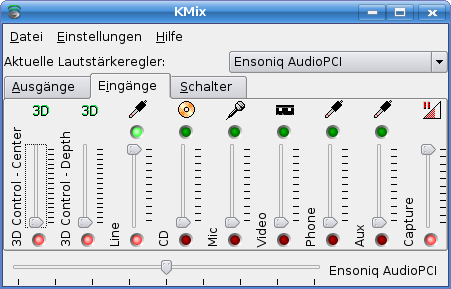
\includegraphics[width=0.75\textwidth]{../images/kmix01.png}
 \caption{Para configurar la tarjeta de audio puede usarse KMix. Asegúrese de que los canales de entrada (Line y Capture) no estén enmudecidos, y que estén dispuestos para grabación (botones verde y rojo).}
 \label{fig_kmix01}
\end{figure}

Cuando esté preparado para grabar, presione el botón \texttt{Grabar} en la barra superior, o teclee CTRL+\sact{ESPACIO}, para comenzar la grabación. Y teclee \sact{ESPACIO} para detenerla. Eso es todo. Para comprobar la grabación, coloque el cursor de reproducción antes de los clips recién creados, y teclee \sact{ESPACIO} para reproducir. Cuando haya terminado de grabar una pista, no olvide desarmarla presionando \sact{A}, o desarme a la vez todas las pistas armadas mediante \dact{A}.


